\section{Wyznaczenie aproksymowanych wektorów $s$ i $s_z$ }
\label{lab:zad3}

\subsection{Odpowiedź skokowa wyjścia od zakłócenia}
\label{lab:zad3:odpSkokZ}

\begin{figure}[H] 
    \centering
    % This file was created by matlab2tikz.
%
\definecolor{mycolor1}{rgb}{0.00000,0.44700,0.74100}%
%
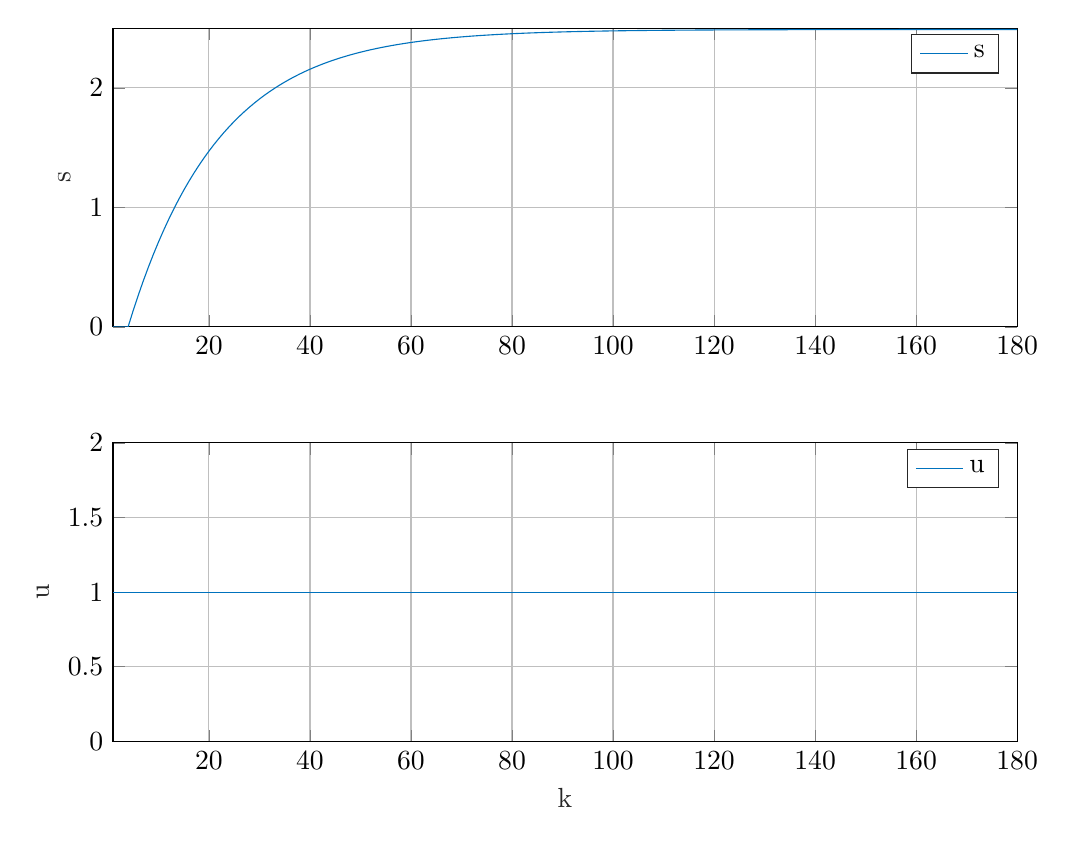
\begin{tikzpicture}

\begin{axis}[%
width=4.521in,
height=1.493in,
at={(0.758in,2.554in)},
scale only axis,
xmin=1,
xmax=180,
ymin=0,
ymax=2.5,
ylabel style={font=\color{white!15!black}},
ylabel={s},
axis background/.style={fill=white},
xmajorgrids,
ymajorgrids,
legend style={legend cell align=left, align=left, draw=white!15!black}
]
\addplot [color=mycolor1]
  table[row sep=crcr]{%
1	0\\
2	0\\
3	0\\
4	0\\
5	0.1351\\
6	0.26289\\
7	0.38377\\
8	0.49811\\
9	0.60625\\
10	0.70854\\
11	0.80528\\
12	0.89678\\
13	0.98332\\
14	1.0652\\
15	1.1426\\
16	1.2158\\
17	1.285\\
18	1.3505\\
19	1.4124\\
20	1.471\\
21	1.5264\\
22	1.5787\\
23	1.6283\\
24	1.6751\\
25	1.7194\\
26	1.7613\\
27	1.8009\\
28	1.8383\\
29	1.8737\\
30	1.9072\\
31	1.9389\\
32	1.9689\\
33	1.9972\\
34	2.024\\
35	2.0493\\
36	2.0732\\
37	2.0959\\
38	2.1173\\
39	2.1375\\
40	2.1567\\
41	2.1748\\
42	2.1919\\
43	2.2081\\
44	2.2234\\
45	2.2379\\
46	2.2516\\
47	2.2645\\
48	2.2768\\
49	2.2883\\
50	2.2993\\
51	2.3096\\
52	2.3194\\
53	2.3286\\
54	2.3374\\
55	2.3457\\
56	2.3535\\
57	2.3609\\
58	2.3679\\
59	2.3745\\
60	2.3807\\
61	2.3866\\
62	2.3922\\
63	2.3975\\
64	2.4025\\
65	2.4072\\
66	2.4117\\
67	2.4159\\
68	2.4199\\
69	2.4237\\
70	2.4273\\
71	2.4307\\
72	2.4339\\
73	2.4369\\
74	2.4397\\
75	2.4424\\
76	2.445\\
77	2.4474\\
78	2.4497\\
79	2.4518\\
80	2.4539\\
81	2.4558\\
82	2.4576\\
83	2.4594\\
84	2.461\\
85	2.4625\\
86	2.464\\
87	2.4654\\
88	2.4667\\
89	2.4679\\
90	2.4691\\
91	2.4702\\
92	2.4712\\
93	2.4722\\
94	2.4731\\
95	2.474\\
96	2.4749\\
97	2.4756\\
98	2.4764\\
99	2.4771\\
100	2.4778\\
101	2.4784\\
102	2.479\\
103	2.4795\\
104	2.4801\\
105	2.4806\\
106	2.4811\\
107	2.4815\\
108	2.4819\\
109	2.4823\\
110	2.4827\\
111	2.4831\\
112	2.4834\\
113	2.4837\\
114	2.484\\
115	2.4843\\
116	2.4846\\
117	2.4849\\
118	2.4851\\
119	2.4853\\
120	2.4856\\
121	2.4858\\
122	2.486\\
123	2.4861\\
124	2.4863\\
125	2.4865\\
126	2.4866\\
127	2.4868\\
128	2.4869\\
129	2.487\\
130	2.4872\\
131	2.4873\\
132	2.4874\\
133	2.4875\\
134	2.4876\\
135	2.4877\\
136	2.4878\\
137	2.4879\\
138	2.4879\\
139	2.488\\
140	2.4881\\
141	2.4882\\
142	2.4882\\
143	2.4883\\
144	2.4883\\
145	2.4884\\
146	2.4884\\
147	2.4885\\
148	2.4885\\
149	2.4886\\
150	2.4886\\
151	2.4887\\
152	2.4887\\
153	2.4887\\
154	2.4888\\
155	2.4888\\
156	2.4888\\
157	2.4889\\
158	2.4889\\
159	2.4889\\
160	2.4889\\
161	2.4889\\
162	2.489\\
163	2.489\\
164	2.489\\
165	2.489\\
166	2.489\\
167	2.4891\\
168	2.4891\\
169	2.4891\\
170	2.4891\\
171	2.4891\\
172	2.4891\\
173	2.4891\\
174	2.4891\\
175	2.4892\\
176	2.4892\\
177	2.4892\\
178	2.4892\\
179	2.4892\\
180	2.4892\\
};
\addlegendentry{s}

\end{axis}

\begin{axis}[%
width=4.521in,
height=1.493in,
at={(0.758in,0.481in)},
scale only axis,
xmin=1,
xmax=180,
xlabel style={font=\color{white!15!black}},
xlabel={k},
ymin=-0,
ymax=2,
ylabel style={font=\color{white!15!black}},
ylabel={u},
axis background/.style={fill=white},
xmajorgrids,
ymajorgrids,
legend style={legend cell align=left, align=left, draw=white!15!black}
]
\addplot[const plot, color=mycolor1] table[row sep=crcr] {%
1	1\\
2	1\\
3	1\\
4	1\\
5	1\\
6	1\\
7	1\\
8	1\\
9	1\\
10	1\\
11	1\\
12	1\\
13	1\\
14	1\\
15	1\\
16	1\\
17	1\\
18	1\\
19	1\\
20	1\\
21	1\\
22	1\\
23	1\\
24	1\\
25	1\\
26	1\\
27	1\\
28	1\\
29	1\\
30	1\\
31	1\\
32	1\\
33	1\\
34	1\\
35	1\\
36	1\\
37	1\\
38	1\\
39	1\\
40	1\\
41	1\\
42	1\\
43	1\\
44	1\\
45	1\\
46	1\\
47	1\\
48	1\\
49	1\\
50	1\\
51	1\\
52	1\\
53	1\\
54	1\\
55	1\\
56	1\\
57	1\\
58	1\\
59	1\\
60	1\\
61	1\\
62	1\\
63	1\\
64	1\\
65	1\\
66	1\\
67	1\\
68	1\\
69	1\\
70	1\\
71	1\\
72	1\\
73	1\\
74	1\\
75	1\\
76	1\\
77	1\\
78	1\\
79	1\\
80	1\\
81	1\\
82	1\\
83	1\\
84	1\\
85	1\\
86	1\\
87	1\\
88	1\\
89	1\\
90	1\\
91	1\\
92	1\\
93	1\\
94	1\\
95	1\\
96	1\\
97	1\\
98	1\\
99	1\\
100	1\\
101	1\\
102	1\\
103	1\\
104	1\\
105	1\\
106	1\\
107	1\\
108	1\\
109	1\\
110	1\\
111	1\\
112	1\\
113	1\\
114	1\\
115	1\\
116	1\\
117	1\\
118	1\\
119	1\\
120	1\\
121	1\\
122	1\\
123	1\\
124	1\\
125	1\\
126	1\\
127	1\\
128	1\\
129	1\\
130	1\\
131	1\\
132	1\\
133	1\\
134	1\\
135	1\\
136	1\\
137	1\\
138	1\\
139	1\\
140	1\\
141	1\\
142	1\\
143	1\\
144	1\\
145	1\\
146	1\\
147	1\\
148	1\\
149	1\\
150	1\\
151	1\\
152	1\\
153	1\\
154	1\\
155	1\\
156	1\\
157	1\\
158	1\\
159	1\\
160	1\\
161	1\\
162	1\\
163	1\\
164	1\\
165	1\\
166	1\\
167	1\\
168	1\\
169	1\\
170	1\\
171	1\\
172	1\\
173	1\\
174	1\\
175	1\\
176	1\\
177	1\\
178	1\\
179	1\\
180	1\\
};
\addlegendentry{u}

\end{axis}
\end{tikzpicture}%
    \caption{Odpowiedź skokowa obiektu od zakłócenia}
    \label{lab:zad3:odpSkokZ:figure}
\end{figure}

\subsection{Aproksymacja odpowiedzi skokowych}
\label{lab:zad3:approxOdpSkok}

Aproksymacja została wykonana jako człon inercyjny drugiego rzędu z opóźnieniem. 
Opisany jest on następującą transmitancją: 

$$G(s)=\frac{K}{(sT_{1}+1)(sT_{2}+1)}e^{-T_{d}s}$$

Powyższa transmitancja po przekształceniu do dziedziny czasu dyskretnego i przejściu na postać równania różnicowego:
%$$G(z)=\frac{z-1}{z}Z\Big[\frac{G(s)}{s})\Big]$$

$$y[k]=b_{1}u[k-T_{D}-1]+b_{2}u[k-T_{D}-2]+a_{1}y[k-1]+a_{2}y[k-2]$$
 
Na podstawie danych pozyskanych ze stanowiska laboratoryjnego dobrano parametry 
$T_{1}$, $T_{2}$, $K$, $T_{d}$, tak aby błąd dopasowania, 
rozumiany jako suma kwadratów kolejnych uchybów sterowania, był jak najmniejszy. 
Należy jednak pamiętać, że wielkość Td może przyjmować tylko wartości całkowite 
(ze względu na zastosowany czas dyskretny). 
W celu doboru parametrów modelu wykorzystano funkcję optymalizacyjną $fmincon$ programu MATLAB, 
jako parametr optymalizacji wybrano błąd dopasowania 
(rozumiany jako suma kwadratów błędów dla kolejnych elementów odpowiedzi skokowych), 
ponieważ im mniejszy błąd dopasowania tym lepsza aproksymacja. \newline
Otrzymane parametry aproksymacji odpowiedzi skokowej od zakłócenia to: \newline
\indent $$T_{1}=\num{7.59}
\indent T_{2}=\num{70.4}
\indent K=\num{0.11}
\indent T_{d}=\num{14.0}$$

\begin{figure}[H] 
    \centering
    % This file was created by matlab2tikz.
%
\definecolor{mycolor1}{rgb}{0.00000,0.44700,0.74100}%
\definecolor{mycolor2}{rgb}{0.85000,0.32500,0.09800}%
%
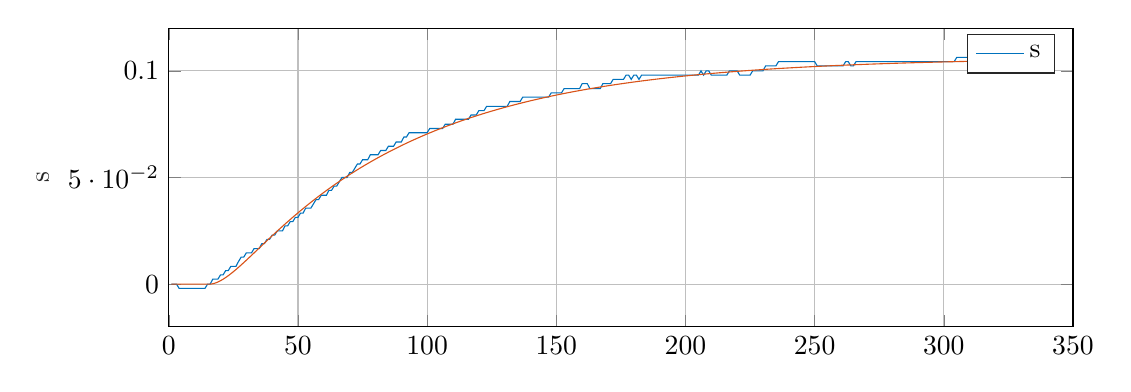
\begin{tikzpicture}

\begin{axis}[%
  width=4.521in,
  height=1.493in,
  at={(0.758in,2.554in)},
scale only axis,
xmin=0,
xmax=350,
ymin=-0.02,
ymax=0.12,
ylabel style={font=\color{white!15!black}},
ylabel={s},
axis background/.style={fill=white},
xmajorgrids,
ymajorgrids,
legend style={legend cell align=left, align=left, draw=white!15!black}
]
\addplot [color=mycolor1]
  table[row sep=crcr]{%
1	0\\
2	0\\
3	0\\
4	-0.00200000000000008\\
5	-0.00200000000000008\\
6	-0.00200000000000008\\
7	-0.00200000000000008\\
8	-0.00200000000000008\\
9	-0.00200000000000008\\
10	-0.00200000000000008\\
11	-0.00200000000000008\\
12	-0.00200000000000008\\
13	-0.00200000000000008\\
14	-0.00200000000000008\\
15	0\\
16	0\\
17	0.00233333333333334\\
18	0.00233333333333334\\
19	0.00233333333333334\\
20	0.00433333333333342\\
21	0.00433333333333342\\
22	0.00633333333333326\\
23	0.00633333333333326\\
24	0.00833333333333333\\
25	0.00833333333333333\\
26	0.00833333333333333\\
27	0.0106666666666667\\
28	0.0126666666666668\\
29	0.0126666666666668\\
30	0.0146666666666666\\
31	0.0146666666666666\\
32	0.0146666666666666\\
33	0.0166666666666667\\
34	0.0166666666666667\\
35	0.0166666666666667\\
36	0.019\\
37	0.019\\
38	0.0210000000000001\\
39	0.0210000000000001\\
40	0.0229999999999999\\
41	0.0229999999999999\\
42	0.025\\
43	0.025\\
44	0.025\\
45	0.0273333333333333\\
46	0.0273333333333333\\
47	0.0293333333333334\\
48	0.0293333333333334\\
49	0.0313333333333333\\
50	0.0313333333333333\\
51	0.0333333333333333\\
52	0.0333333333333333\\
53	0.0356666666666667\\
54	0.0356666666666667\\
55	0.0356666666666667\\
56	0.0376666666666668\\
57	0.0396666666666666\\
58	0.0396666666666666\\
59	0.0416666666666667\\
60	0.0416666666666667\\
61	0.0416666666666667\\
62	0.044\\
63	0.044\\
64	0.0460000000000001\\
65	0.0460000000000001\\
66	0.0479999999999999\\
67	0.05\\
68	0.05\\
69	0.05\\
70	0.0523333333333333\\
71	0.0523333333333333\\
72	0.0543333333333334\\
73	0.0563333333333333\\
74	0.0563333333333333\\
75	0.0583333333333333\\
76	0.0583333333333333\\
77	0.0583333333333333\\
78	0.0606666666666667\\
79	0.0606666666666667\\
80	0.0606666666666667\\
81	0.0606666666666667\\
82	0.0626666666666667\\
83	0.0626666666666667\\
84	0.0626666666666667\\
85	0.0646666666666666\\
86	0.0646666666666666\\
87	0.0646666666666666\\
88	0.0666666666666667\\
89	0.0666666666666667\\
90	0.0666666666666667\\
91	0.069\\
92	0.069\\
93	0.0710000000000001\\
94	0.0710000000000001\\
95	0.0710000000000001\\
96	0.0710000000000001\\
97	0.0710000000000001\\
98	0.0710000000000001\\
99	0.0710000000000001\\
100	0.0710000000000001\\
101	0.0729999999999999\\
102	0.0729999999999999\\
103	0.0729999999999999\\
104	0.0729999999999999\\
105	0.0729999999999999\\
106	0.0729999999999999\\
107	0.075\\
108	0.075\\
109	0.075\\
110	0.075\\
111	0.0773333333333333\\
112	0.0773333333333333\\
113	0.0773333333333333\\
114	0.0773333333333333\\
115	0.0773333333333333\\
116	0.0773333333333333\\
117	0.0793333333333334\\
118	0.0793333333333334\\
119	0.0793333333333334\\
120	0.0813333333333333\\
121	0.0813333333333333\\
122	0.0813333333333333\\
123	0.0833333333333333\\
124	0.0833333333333333\\
125	0.0833333333333333\\
126	0.0833333333333333\\
127	0.0833333333333333\\
128	0.0833333333333333\\
129	0.0833333333333333\\
130	0.0833333333333333\\
131	0.0833333333333333\\
132	0.0856666666666667\\
133	0.0856666666666667\\
134	0.0856666666666667\\
135	0.0856666666666667\\
136	0.0856666666666667\\
137	0.0876666666666668\\
138	0.0876666666666668\\
139	0.0876666666666668\\
140	0.0876666666666668\\
141	0.0876666666666668\\
142	0.0876666666666668\\
143	0.0876666666666668\\
144	0.0876666666666668\\
145	0.0876666666666668\\
146	0.0876666666666668\\
147	0.0876666666666668\\
148	0.0896666666666666\\
149	0.0896666666666666\\
150	0.0896666666666666\\
151	0.0896666666666666\\
152	0.0896666666666666\\
153	0.0916666666666667\\
154	0.0916666666666667\\
155	0.0916666666666667\\
156	0.0916666666666667\\
157	0.0916666666666667\\
158	0.0916666666666667\\
159	0.0916666666666667\\
160	0.094\\
161	0.094\\
162	0.094\\
163	0.0916666666666667\\
164	0.0916666666666667\\
165	0.0916666666666667\\
166	0.0916666666666667\\
167	0.0916666666666667\\
168	0.094\\
169	0.094\\
170	0.094\\
171	0.094\\
172	0.0960000000000001\\
173	0.0960000000000001\\
174	0.0960000000000001\\
175	0.0960000000000001\\
176	0.0960000000000001\\
177	0.0979999999999999\\
178	0.0979999999999999\\
179	0.0960000000000001\\
180	0.0979999999999999\\
181	0.0979999999999999\\
182	0.0960000000000001\\
183	0.0979999999999999\\
184	0.0979999999999999\\
185	0.0979999999999999\\
186	0.0979999999999999\\
187	0.0979999999999999\\
188	0.0979999999999999\\
189	0.0979999999999999\\
190	0.0979999999999999\\
191	0.0979999999999999\\
192	0.0979999999999999\\
193	0.0979999999999999\\
194	0.0979999999999999\\
195	0.0979999999999999\\
196	0.0979999999999999\\
197	0.0979999999999999\\
198	0.0979999999999999\\
199	0.0979999999999999\\
200	0.0979999999999999\\
201	0.0979999999999999\\
202	0.0979999999999999\\
203	0.0979999999999999\\
204	0.0979999999999999\\
205	0.0979999999999999\\
206	0.1\\
207	0.0979999999999999\\
208	0.1\\
209	0.1\\
210	0.0979999999999999\\
211	0.0979999999999999\\
212	0.0979999999999999\\
213	0.0979999999999999\\
214	0.0979999999999999\\
215	0.0979999999999999\\
216	0.0979999999999999\\
217	0.1\\
218	0.1\\
219	0.1\\
220	0.1\\
221	0.0979999999999999\\
222	0.0979999999999999\\
223	0.0979999999999999\\
224	0.0979999999999999\\
225	0.0979999999999999\\
226	0.1\\
227	0.1\\
228	0.1\\
229	0.1\\
230	0.1\\
231	0.102333333333333\\
232	0.102333333333333\\
233	0.102333333333333\\
234	0.102333333333333\\
235	0.102333333333333\\
236	0.104333333333333\\
237	0.104333333333333\\
238	0.104333333333333\\
239	0.104333333333333\\
240	0.104333333333333\\
241	0.104333333333333\\
242	0.104333333333333\\
243	0.104333333333333\\
244	0.104333333333333\\
245	0.104333333333333\\
246	0.104333333333333\\
247	0.104333333333333\\
248	0.104333333333333\\
249	0.104333333333333\\
250	0.104333333333333\\
251	0.102333333333333\\
252	0.102333333333333\\
253	0.102333333333333\\
254	0.102333333333333\\
255	0.102333333333333\\
256	0.102333333333333\\
257	0.102333333333333\\
258	0.102333333333333\\
259	0.102333333333333\\
260	0.102333333333333\\
261	0.102333333333333\\
262	0.104333333333333\\
263	0.104333333333333\\
264	0.102333333333333\\
265	0.102333333333333\\
266	0.104333333333333\\
267	0.104333333333333\\
268	0.104333333333333\\
269	0.104333333333333\\
270	0.104333333333333\\
271	0.104333333333333\\
272	0.104333333333333\\
273	0.104333333333333\\
274	0.104333333333333\\
275	0.104333333333333\\
276	0.104333333333333\\
277	0.104333333333333\\
278	0.104333333333333\\
279	0.104333333333333\\
280	0.104333333333333\\
281	0.104333333333333\\
282	0.104333333333333\\
283	0.104333333333333\\
284	0.104333333333333\\
285	0.104333333333333\\
286	0.104333333333333\\
287	0.104333333333333\\
288	0.104333333333333\\
289	0.104333333333333\\
290	0.104333333333333\\
291	0.104333333333333\\
292	0.104333333333333\\
293	0.104333333333333\\
294	0.104333333333333\\
295	0.104333333333333\\
296	0.104333333333333\\
297	0.104333333333333\\
298	0.104333333333333\\
299	0.104333333333333\\
300	0.104333333333333\\
301	0.104333333333333\\
302	0.104333333333333\\
303	0.104333333333333\\
304	0.104333333333333\\
305	0.106333333333333\\
306	0.106333333333333\\
307	0.106333333333333\\
308	0.106333333333333\\
309	0.106333333333333\\
310	0.106333333333333\\
311	0.106333333333333\\
312	0.106333333333333\\
313	0.106333333333333\\
314	0.106333333333333\\
315	0.106333333333333\\
316	0.106333333333333\\
};
\addlegendentry{s}

\addplot [color=mycolor2, forget plot]
  table[row sep=crcr]{%
1	0\\
2	0\\
3	0\\
4	0\\
5	0\\
6	0\\
7	0\\
8	0\\
9	0\\
10	0\\
11	0\\
12	0\\
13	0\\
14	0\\
15	0\\
16	0\\
17	0.000185072726593913\\
18	0.000529762157235997\\
19	0.00101179142541201\\
20	0.00161166986027936\\
21	0.00231234854140959\\
22	0.00309891837973291\\
23	0.00395834547506707\\
24	0.00487923914863741\\
25	0.00585164861702559\\
26	0.00686688477189672\\
27	0.00791736396630322\\
28	0.00899647109093682\\
29	0.0100984395590469\\
30	0.011218246112695\\
31	0.0123515186206803\\
32	0.0134944552643298\\
33	0.0146437537053256\\
34	0.0157965490032791\\
35	0.0169503592028822\\
36	0.0181030376438027\\
37	0.0192527311633722\\
38	0.0203978434645666\\
39	0.0215370030115851\\
40	0.0226690348940507\\
41	0.0237929361698612\\
42	0.0249078542571998\\
43	0.0260130679992361\\
44	0.0271079710715184\\
45	0.0281920574427976\\
46	0.0292649086357297\\
47	0.0303261825652036\\
48	0.0313756037594771\\
49	0.032412954793356\\
50	0.0334380687837283\\
51	0.0344508228162469\\
52	0.0354511321881499\\
53	0.0364389453664071\\
54	0.0374142395728253\\
55	0.0383770169186555\\
56	0.0393273010208055\\
57	0.0402651340401466\\
58	0.0411905740897459\\
59	0.0421036929673015\\
60	0.0430045741716982\\
61	0.0438933111685524\\
62	0.0447700058739529\\
63	0.0456347673294039\\
64	0.0464877105443123\\
65	0.0473289554852807\\
66	0.0481586261940279\\
67	0.0489768500180066\\
68	0.0497837569397504\\
69	0.0505794789927122\\
70	0.0513641497528626\\
71	0.0521379038966476\\
72	0.052900876817061\\
73	0.0536532042906086\\
74	0.0543950221888332\\
75	0.0551264662288497\\
76	0.055847671758028\\
77	0.0565587735685614\\
78	0.0572599057381829\\
79	0.0579512014937577\\
80	0.0586327930948822\\
81	0.0593048117349739\\
82	0.0599673874576511\\
83	0.0606206490864698\\
84	0.0612647241663269\\
85	0.0618997389150483\\
86	0.0625258181838602\\
87	0.06314308542561\\
88	0.0637516626697359\\
89	0.0643516705031151\\
90	0.0649432280560237\\
91	0.0655264529925401\\
92	0.0661014615048034\\
93	0.0666683683106152\\
94	0.0672272866539331\\
95	0.0677783283078643\\
96	0.0683216035798122\\
97	0.0688572213184768\\
98	0.0693852889224439\\
99	0.0699059123501322\\
100	0.0704191961308975\\
101	0.0709252433771164\\
102	0.0714241557970963\\
103	0.0719160337086766\\
104	0.0724009760534037\\
105	0.0728790804111772\\
106	0.0733504430152778\\
107	0.0738151587676982\\
108	0.0742733212547111\\
109	0.0747250227626123\\
110	0.0751703542935904\\
111	0.0756094055816759\\
112	0.0760422651087328\\
113	0.0764690201204589\\
114	0.0768897566423643\\
115	0.0773045594957058\\
116	0.0777135123133523\\
117	0.0781166975555663\\
118	0.0785141965256825\\
119	0.0789060893856721\\
120	0.0792924551715803\\
121	0.0796733718088276\\
122	0.0800489161273669\\
123	0.0804191638766892\\
124	0.0807841897406728\\
125	0.0811440673522712\\
126	0.0814988693080356\\
127	0.0818486671824703\\
128	0.0821935315422174\\
129	0.08253353196007\\
130	0.0828687370288128\\
131	0.0831992143748894\\
132	0.0835250306718956\\
133	0.0838462516538994\\
134	0.0841629421285881\\
135	0.0844751659902422\\
136	0.0847829862325382\\
137	0.0850864649611807\\
138	0.0853856634063644\\
139	0.0856806419350687\\
140	0.0859714600631851\\
141	0.0862581764674798\\
142	0.086540848997392\\
143	0.0868195346866712\\
144	0.0870942897648534\\
145	0.08736516966858\\
146	0.0876322290527585\\
147	0.08789552180157\\
148	0.088155101039323\\
149	0.0884110191411563\\
150	0.0886633277435924\\
151	0.0889120777549443\\
152	0.0891573193655763\\
153	0.0893991020580219\\
154	0.0896374746169588\\
155	0.0898724851390461\\
156	0.0901041810426215\\
157	0.0903326090772639\\
158	0.0905578153332212\\
159	0.0907798452507056\\
160	0.0909987436290584\\
161	0.091214554635786\\
162	0.0914273218154689\\
163	0.0916370880985449\\
164	0.0918438958099695\\
165	0.0920477866777536\\
166	0.0922488018413815\\
167	0.0924469818601101\\
168	0.0926423667211514\\
169	0.0928349958477398\\
170	0.0930249081070853\\
171	0.0932121418182153\\
172	0.0933967347597051\\
173	0.0935787241773002\\
174	0.0937581467914312\\
175	0.0939350388046215\\
176	0.0941094359087925\\
177	0.0942813732924642\\
178	0.0944508856478553\\
179	0.0946180071778825\\
180	0.0947827716030618\\
181	0.0949452121683118\\
182	0.0951053616496615\\
183	0.0952632523608638\\
184	0.0954189161599146\\
185	0.0955723844554814\\
186	0.0957236882132403\\
187	0.0958728579621239\\
188	0.0960199238004813\\
189	0.0961649154021507\\
190	0.096307862022447\\
191	0.0964487925040645\\
192	0.0965877352828966\\
193	0.0967247183937732\\
194	0.0968597694761176\\
195	0.0969929157795227\\
196	0.0971241841692502\\
197	0.0972536011316501\\
198	0.0973811927795059\\
199	0.0975069848573026\\
200	0.0976310027464219\\
201	0.0977532714702629\\
202	0.0978738156992915\\
203	0.0979926597560179\\
204	0.0981098276199045\\
205	0.0982253429322042\\
206	0.0983392290007302\\
207	0.0984515088045595\\
208	0.0985622049986688\\
209	0.0986713399185062\\
210	0.0987789355844975\\
211	0.0988850137064893\\
212	0.0989895956881299\\
213	0.0990927026311872\\
214	0.0991943553398074\\
215	0.0992945743247118\\
216	0.0993933798073359\\
217	0.0994907917239092\\
218	0.0995868297294779\\
219	0.0996815132018709\\
220	0.0997748612456094\\
221	0.0998668926957619\\
222	0.0999576261217444\\
223	0.100047079831068\\
224	0.10013527187303\\
225	0.100222220042362\\
226	0.100307941882812\\
227	0.10039245469069\\
228	0.100475775518359\\
229	0.100557921177669\\
230	0.100638908243356\\
231	0.100718753056383\\
232	0.100797471727238\\
233	0.100875080139185\\
234	0.100951593951466\\
235	0.101027028602466\\
236	0.101101399312823\\
237	0.1011747210885\\
238	0.101247008723818\\
239	0.101318276804432\\
240	0.101388539710282\\
241	0.101457811618491\\
242	0.101526106506224\\
243	0.101593438153512\\
244	0.101659820146031\\
245	0.10172526587784\\
246	0.10178978855409\\
247	0.101853401193683\\
248	0.101916116631899\\
249	0.10197794752299\\
250	0.10203890634273\\
251	0.102099005390932\\
252	0.102158256793932\\
253	0.102216672507033\\
254	0.102274264316922\\
255	0.10233104384404\\
256	0.102387022544936\\
257	0.102442211714572\\
258	0.102496622488605\\
259	0.102550265845633\\
260	0.102603152609411\\
261	0.102655293451034\\
262	0.102706698891089\\
263	0.102757379301781\\
264	0.102807344909024\\
265	0.102856605794503\\
266	0.10290517189771\\
267	0.10295305301795\\
268	0.103000258816316\\
269	0.103046798817641\\
270	0.103092682412416\\
271	0.10313791885869\\
272	0.103182517283934\\
273	0.103226486686883\\
274	0.103269835939355\\
275	0.103312573788036\\
276	0.10335470885625\\
277	0.103396249645694\\
278	0.103437204538157\\
279	0.103477581797211\\
280	0.103517389569877\\
281	0.103556635888268\\
282	0.103595328671213\\
283	0.10363347572585\\
284	0.103671084749208\\
285	0.103708163329752\\
286	0.10374471894892\\
287	0.103780758982632\\
288	0.103816290702776\\
289	0.103851321278675\\
290	0.103885857778536\\
291	0.103919907170877\\
292	0.103953476325926\\
293	0.103986572017019\\
294	0.104019200921953\\
295	0.104051369624347\\
296	0.104083084614958\\
297	0.104114352293001\\
298	0.104145178967433\\
299	0.104175570858228\\
300	0.104205534097637\\
301	0.104235074731415\\
302	0.10426419872005\\
303	0.104292911939964\\
304	0.104321220184694\\
305	0.104349129166065\\
306	0.104376644515342\\
307	0.104403771784368\\
308	0.104430516446677\\
309	0.104456883898609\\
310	0.104482879460389\\
311	0.104508508377208\\
312	0.104533775820276\\
313	0.104558686887868\\
314	0.104583246606353\\
315	0.104607459931206\\
316	0.104631331748012\\
};
\end{axis}
\end{tikzpicture}%
    \caption{Aproksymowana odpowiedź skokowa od zakłócenia}
    \label{lab:zad3:approxOdpSkokZ:figure}
\end{figure}

\newpage
